% Introductory paragraph.
A wide variety of data sources were used in order to populate all KiPhoDB tables.
In this section we will examine each external database that we used for this purpose by providing a brief description of it and listing its advantages and disadvantages.
In addition to that, we will also explain which parts of the external data source were most useful and how we utilized them in order to achieve our target.

% PhosphoELM
\section{PhosphoELM}
PhosphoELM \cite{phosphoELM} is a database that contains eukaryotic phosphorylation sites and it is available online at http://phospho.elm.eu.org.
All database entries are manually curated and the data were collected both from published scientific literature and high-throughput data sets.
It provides information not only about the exact phosphorylation sites of each protein, but also the kinases that are responsible for each post-translational modification.
Moreover it includes numerous links to bibliographic references and a lot of additional information about interaction partners, structures, etc.
From the above description it would appear that PhosphoELM is a good data resource that contains high quality and experimentally verified data and therefore should be one
of the primary information sources for the creation of KiPhoDB.

Numerous bioinformatics projects have used the PhosphoELM data set in the past.
Some of these are for example the kinase-specific prediction server GPS (Group-based Phosphorylation Scoring) \cite{gps},
the literature mining rule-based program RLIMS-P \cite{rlims-p}, the database of tissue and phosphoprotein sub-cellular distribution PhoshporegDB \cite{phosphoregdb} 
and many more.
This seems to indicate that the PhosphoELM database is widely accepted in the bioinformatics community as a reliable resource of phosphorylation site data and therefore it is safe to use it as one of the primary data sources for KiPhoDB.

We used the latest version of this database (version 8.1), which was released in December 2008.
According to the release notes, this version contains 4384 protein entries (2166 Tyrosine, 13320 Serine and 2766 Threonine), with more than 18,000 phosphorylation sites.
The vast majority of these proteins and phosphorylation sites come from two species: human and mouse.
The reason why these two species are prevalent in the PhosphoELM database is that they are both used extensively as model organisms in biological research.

One other significant characteristic of PhosphoELM is that for each phosphosite the database reports if the phosphorylation evidence originates from small-scale analysis
(LTP - low-throughput) or large-scale experiments (HTP - high-throughput).
LTP experiments typically focus on a limited number of proteins at a time, whereas HTP methodologies and techniques, such as mass spectrometry, examine a great number of proteins each time.
In the PhosphoELM data set there is a small overlap between phosphosites identified by LTP and HTP experiments \cite{phosphoELM}.
Therefore we had to be very careful while using the data to enrich the contents of KiPhoDB and take all necessary actions so that each phosphorylation site would be inserted only once in our database.

One final characteristic of PhosphoELM that is worth mentioning is that the kinase enzyme responsible for phosphorylation is known for only about 21\% of substrates.
The latest version of PhosphoELM. that we have used in this project contains more than 250 kinases, but the majority of them refer to a general category of kinase enzymes and not to a specific kinase protein of a certain species.
As a consequence, although PhosphoELM is an excellent resource for substrates and exact phosphorylation sites, it provides very limited information concerning the exact kinase enzyme that is responsible for each phosphorylation.
In order to obtain this kind of information and insert it into our database, we had to resort to other databases and data sources, which will be described in detail in the following sections.

% NetworKIN
\section{NetworKIN}
NetworKIN is a methodology for predicting in vivo kinase-substrate relationships.
Its main aim is to find a systematic way to link experimentally verified phosphorylation sites to protein kinases.
In order to achieve this, it exploits the fact that signaling proteins contain various catalytic or interaction domains and phosphorylation or binding motifs that play a major role in protein interactions.
Additionally, it also utilizes the ability of certain kinase catalytic domains to phosphorylate particular sequence motifs and contextual information concerning the cooccurrence in the literature, physical association and coexpression of kinases and substrates.
The project's website can be found at http://networking.info and it allows users to browse and search predictions made by the NetworKIN algorithm.

According to the NetworKIN publication \cite{networKIN}, the algorithm augments motif-based prediction by taking into consideration the network of kinases and phosphoproteins, leading to an overall improvement in the accuracy with which phosphorylation networks can be build.
In more detail, it tries to predict which protein kinases target experimentally identified phosphorylation sites by combining protein association networks with consensus sequence motifs.
At first, the NetworKIN algorithm uses neural networks and PSMs (Position-specific Scoring Matrices) in order to determine which kinase family phosphorylates each phospho-site.
Subsequently the STRING database is queried in order to construct a probabilistic protein network for every substrate, which contains a lot of contextual information that can significantly improve the final prediction.
This contextual information includes for example manually curated pathway data, mRNA expression studies, coocurence in abstracts and genomic context.
At the end, the algorithm produces predictions based on sequence similarity searches against a database of kinase domain sequences.
Further information about the exact function of the NetworKIN algorithm can be found in \cite{networKIN}.

We have chosen to use NetworKIN as one of our data sources because it has a lot of advantages.
One of these advantages is that it is able to capture both direct and indirect interactions between kinases and the corresponding substrates, which enables the algorithm to produce non-obvious predictions that would otherwise be very difficult to make.
One other advantage of NetworKIN is its relatively high accuracy, compared to other algorithms that use only consensus motifs.
According to \cite{networKIN} the algorithm's accuracy is approximately 64\%, which is a 2.5 fold improvement comparing to other algorithms offering a maximum accuracy of 25\%.
Finally, the third reason that led us into choosing NetworKIN as one of our data sources is its close collaboration and integration with PhosphoELM.
NetworKIN has been applied to the PhosphoELM data set at the past, producing very accurate results and enabling scientists to construct an approximation of the whole phosphatase and kinase interaction network for humans.
Therefore it is essential to include this information in the KiPhoDB database, as it will enrich its contents even further.

The major problem that we had to face while using the NetworKIN data stems from the fact that this algorithm generates predictions which, although relatively accurate, can be false.
Therefore we had to include additional fields in the KiPhoDB database that would store the probability of each prediction being true and thus give a measure of confidence to the database user.
It is then the user's responsibility to accept or ignore the prediction.
In addition to this measure, we also had to discard some of the data coming from the NetworKIN database because their significance was rather low.
We tried to keep only those data whose quality was high.
In this way we tightly controlled the quality of data entering our database and thus we managed to keep the high standards that we initially aimed for.

\begin{figure}[htp]
\centering
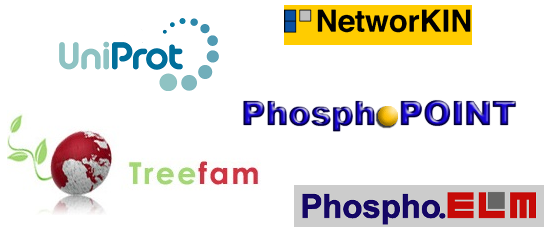
\includegraphics[scale=0.6]{pictures/DataSourcesLogos.png}
\caption{Some of the data sources used in this project.}
\label{DataSourcesLogos}
\end{figure}

%Phosida
\section{Phosida}
Phosida is a phosphorylation site database which can be found at http://www.phosida.com.
It contains numerous high-confidence phosphosites from a great variety of species, which have been positively identified in vivo using high resolution mass spectrometry techniques.
As its creators argue in \cite{PHOSIDA}, the use of high resolution mass spectrometry has an estimated false positive rate of less than one percent.
The previous statement proves that Phosida contains very high quality data and therefore should be used in order to populate the KiPhoDB database.
Furthermore, Phosida also provides information about the evolution of phosphorylation sites by examining similar phosphoproteins in different eukaryotic and prokaryotic organisms.
Finally, it also integrates a phosphosite prediction algorithm, which uses SVM (Support Vector Machines) to predict the existence of phosphorylation sites in non-annotated protein sequences.

The aforementioned phosphosite predictor takes advantage of the numerous in vivo identified phosphosites that the Phosida database contains in order to find novel phosphorylation sites that have not previously been identified.
This process produces predictions that can be used to estimate a protein's role in a pathway or its involvement in a signaling cascade and design other biological experiments that will uncover its true functionality and validate or discard the predictions.
Finally the prediction algorithm enables users to specify certain precision and recall levels so that the predictions will have a high probability of being true.
Of course we did not use the predictor to insert data in our database, because we wanted KiPhoDB to contain only data that have been experimentally proven and not predicted phosphorylation sites or proteins.

Phosida was initially developed in order to store phosphosite information from large scale quantitative experiments and thus it contains many quantitative data which were not relevant to the purpose of this database project.
For example, for each protein the database contains its molecular weight, its isoelectric point (pI)  and many more information in addition to all phosphorylation sites that have been identified on it \cite{PHOSIDA}.
Moreover, for each phosphorylation site Phosida contains its predicted secondary structure, matching kinase motifs and conservation patterns.
KiPhoDB utilizes only part of this information, because we did not want to include all this biological context but only the data that was most useful to the database users.

%PhosphoPOINT
\section{PhosphoPOINT}
PhosphoPOINT is a human kinase interactome database, which aims to provide information and shed light on the interactome of 518 human protein kinases, their potential substrates and interacting partners.
It integrates information from three existing phosphoprotein databases, namely PhosphoELM, HPRD and Swissprot, as well as approximately 400 manually curated kinase - substrate pairs.
It is constantly updated as soon as new versions of the aforementioned databases are released.
At the time of writing, it contains 4195 phosphoproteins with a total of 15,738 phosphorylation sites (10,937 Serine, 2,425 Threonine and 2,376 Tyrosine) and it is available at http://kinase.bioinformatics.tw.
7,843 of these phosphorylation sites come from high-throughput (HTP) experiments, 6,329 come from low-throughput (LTP) experiments and 679 come from both HTP and LTP screening.
The above information will help us judge the quality of the data in the PhosphoPOINT database and decide whether we will use it as a data source for KiPhoDB or not.

In addition to kinase - substrate pairs for human kinases, the PhosphoPOINT database also provides all adequate annotation that helps scientists locate new kinase - substrate pairs using the available protein-protein interaction data sets.
Moreover, Gene Ontology (GO) \cite{go} cellular component information and external gene expression data sets are used to identify potential substrates for each kinase.
Finally, PhosphoPOINT provides annotation to some of the amino acids located near each phosphorylation site, where a Single Nucleotide Polymorphism can cause the corruption of this site.
This information can be very helpful and provide insight on how such alterations lead to the emergence of human disease.
For example it has been found \cite{PhosphoPoint} that there are at least 64 phosphorylation sites whose change results to disease phenotypes such as schizophrenia and hypertension.

\begin{table}[h]
\vspace{1cm}
\begin{center}
\begin{tabular}{ | c | c | }
\hline
\textbf{Category} & \textbf{Explanation} \\
\hline
\hline
1 & physically interacting proteins \\
\hline
2 & interacting phosphoproteins \\
\hline
3 & substrates for a biochemical reaction \\
\hline
4 & substrates \& interacting phosphoproteins \\
\hline
\end{tabular}
\end{center}
\caption{The different categories of data in PhosphoPOINT.}
\label{table:PhosphoPoint1}
\vspace{1cm}
\end{table}

According to \cite{PhosphoPoint}, there are four kinds of links between kinases and their interacting substrates, as it is clearly illustrated in Table \ref{table:PhosphoPoint1}.
All interactions available in the PhosphoPOINT database are classified into one of these categories.
For the purpose of populating our database, we have chosen to use only categories three (substrates for a biochemical reaction) and four (substrates \& interacting phosphoproteins).
Categories one (physically interacting proteins) and two (interacting phosphoproteins) contain interacting proteins in general, which means that they may contain proteins that do not undergo phosphorylation but some other kind of interaction.
Therefore we decided not to use categories one and two and limit the available dataset to the remaining two categories, which undoubtedly contain substrates that participate in phosphorylation reactions.

% PhosphaBase
\section{PhosphaBase}
PhosphaBase was used in this project as a primary resource for phosphatase information and it can be found at http://www.bioinf.manchester.ac.uk/phosphabase/.
It currently contains 11445 number of sequences belonging to 1112 organisms \cite{phosphabase}.
The exact contents of PhosphaBase are illustrated in more detail in Table \ref{table:PhosphaBase}.
It is an ontology-driven database and the first public resource dedicated to protein phosphatases.
The data found inside PhosphaBase have been collected from a great variety of biological sources, such as peer-reviewed literature and other publicly available biological databases (Uniprot, PDB, etc).
Moreover, Gene Ontology terms have been used as a means of data extraction, in order to eliminate redundancy in the final data set.

\begin{table}[h]
\vspace{1cm}
\begin{center}
\begin{tabular} {|l|c|}
\hline
\textbf{Phosphatase Subfamily} & \textbf{Number of Sequences}\\
\hline
\hline
Protein tyrosine phosphatases & 2598 \\
\hline
Dual-specificity phosphatases & 1360\\
\hline
PTEN and Myotubularins & 233\\
\hline
Serine/Threonine phosphatases & 6370\\
\hline
Histidine phosphatases & 47\\
\hline
Unclassified serine/threonine phosphatases & 154\\
\hline
Unclassified tyrosine phosphatases & 683\\
\hline
\hline
Total & 11445\\
\hline
\end{tabular}
\end{center}
\caption{The current contents of PhosphaBase.}
\label{table:PhosphaBase}
\vspace{1cm}
\end{table}

In general, PhosphaBase contains very useful data of acceptable quality.
Although the developers of PhosphaBase have put a lot of effort in eliminating redundancy in the data set, there are some cases where search results will contain duplicated information.
This happens because no manual curation is performed on the database and therefore there is no way to delete duplicate entries that have been initially created due to the inability of computer programs to detect and prevent this kind of errors.
In addition to that, some false positives have been reported when a protein listed in PhosphaBase is not actually a phosphatase.
This can happen when a protein has a specific domain that is normally found on phosphatases but does not exhibit phosphatase behaviour.
One positive fact though is that PhosphaBase does not contain any protein sequence fragments and therefore the redundancy problems that fragments may cause have been successfully avoided.

Taking under serious consideration the negative characteristics of PhosphaBase that where presented in the previous paragraph, we decided to include it as one of our data sources for phosphatases.
This decision was mainly affected by the fact that there exist very few databases for phosphatases and thus we had to use all available information for this kind of molecules.
Nevertheless, we took all necessary steps in order to actively control the data inserted in KiPhoDB by performing regular checks and discarding those data that appeared to be redundant.

% KinBase
\section{KinBase}
KinBase is a database that contains data for all protein kinase genes found in various species.
The species that are currently covered by KinBase are the following: Human, Mouse, Sea Urchin, Fruit Fly (Drosophila melanogaster), Nematode Worm (C. elegans), Monosiga brevicollis, Yeast (S. cerevisiae), Dictyostelium and Tetrahymena.
KinBase is available at http://kinase.com/kinbase/ and it is searchable by kinase group, family, subfamily, gene name and domain.
Finally, the KinBase website integrates a BLAST server, which can be utilized in order to perform sequence similarity searches.

In this project we have used KinBase as a supplementary resource for kinase data.
One characteristic of the KinBase database is that it contains information about pseudokinases.
This category of kinases corresponds to about 10\% of the total number of kinases in humans and they are predicted to be non-functional due to evolutionary changes in important amino acids of the protein sequence.
Although pseudokinases are inactive and they do not function as proper kinase enzymes, they are thought to retain other roles in the cell that
render them essential for its function \cite{pseudokinases}.
Therefore we had to be very careful when using this data source and filter out all pseudokinases, because they are not relevant to our targets in this project and thus they should not be included into the KiPhoDB database.

%NetPath
\section{NetPath}
NetPath is a curated data source that contains valuable information about signal transduction pathways in humans.
It can be found at http://www.netpath.org and its current contents are listed in Table \ref{table:Netpath}.
At the moment it contains a total of twenty pathways, which are freely available to download.
Ten of these pathways concern immune signaling, whereas the remaining ten are cancer signaling pathways.
The data contained in NetPath are mainly from humans, but the database contains information from other mammals too.
Until now signaling pathways have been studied with focus on isolated members or individual reactions and no comprehensive view of the pathway as a whole was possible.
Netpath's main characteristic is that it provides a global view of pathways, including many details of protein-protein interactions, enzyme catalysis, translocation of proteins etc.
Moreover, its main source of data is HPRD, the Human Protein Reference Database.

\begin{table}
\vspace{1cm}
\begin{center}
\begin{tabular} {|l|c|}
\hline
\textbf{Category} & \textbf{Contents}\\
\hline
\hline
Curated Pathways & 20\\
\hline
Molecules & 963\\
\hline
Physical Interactions & 1649\\
\hline
Genes Transcriptionally Regulated & 6137\\
\hline
Transport & 148\\
\hline
Enzyme Catalysis & 729\\
\hline
PubMed Citations & 10209\\
\hline
\end{tabular}
\end{center}
\caption{The current contents of NetPath.}
\label{table:Netpath}
\vspace{1cm}
\end{table}

We exploited this website by downloading the available NetPath data set in BioPAX format and trying to identify phosphorylation and dephosphorylation reactions between proteins in various pathways.
Using this information we managed to pinpoint certain kinase-substrate and phosphatase-substrate pairs and identify kinases and phosphatases that act on the same substrate.
However, as expected, the number of phosphatase-substrate pairs that were finally discovered, were far less than the kinase - substrate pairs.

%Treefam
\section{TreeFam}
TreeFam is a phylogenetic tree database which can be found at http://www.treefam.org \cite{treefam1}.
It consists of two distinct parts.
The first part is named Treefam-A and it includes manually curated phylogenetic trees for 1314 gene families.
In contrast, the second part consists of automatically generated phylogenetic trees for 14351 families and it is called Treefam-B.
A gene family can be thought of as a group of genes that have high sequence similarity because they have descended from a single gene in the last common ancestor.
In order to populate the KiPhoDB database, we used the fourth version of Treefam which includes 25 fully sequenced animal genomes,
along with four genomes from plant and fungal species.

Phylogenetic trees offered by TreeFam are very useful for scientists because they can be exploited in order to identify orthologous (originating from speciation) and paralogous (originating from duplication) genes.
Therefore useful assumptions can be formed about the relationship between corresponding genes in different organisms, which can help us shed some light into the evolutionary history of genes and gain a deeper understanding of the evolution of organisms and their genomes.
One other way to obtain this kind of information is by using BLAST matches (Inparanoid, KOG) or BLAST matches and synteny (HomoloGene, Ensembl-Compara).
As the creators of TreeFam claim in \cite{treefam2}, tree-based inference of paralogs and orthologs is a much more robust and accurate technique for many reasons.
The primary one being that pair-wise BLAST scores are greatly affected by the difference of evolutionary rates between members of the same gene family.
On the other hand, phylogenetic trees do not have this problem and they are much more informative because they can visually illustrate the history of a whole gene family.
Finally, another positive aspect of phylogenetic trees is that they offer scientists the opportunity to compare gene trees and species trees and draw useful conclusions.

We have used the TreeFam data source in order to obtain information about kinase and phosphatase gene families.
As noted previously, TreeFam contains two separate data sets: TreeFam-A and TreeFam-B.
The trees included in TreeFam-B are automatically generated and therefore they are often incorrect because of poor data quality and certain faults in the tree generation algorithms.
For more details about the algorithms that TreeFam uses in order to automatically produce phylogenetic trees, infer orthologue or paralogue relationships and classify genes into families can be found in \cite{treefam1}.
Since the data in TreeFam-B data set are prone to errors, we decided to only use TreeFam-A.
Thus we only inserted manually curated trees in our database in the hope of conserving the relatively high quality standard of the data provided by KiPhoDB.

\section{Other resources}
Apart from the data sources that were described in previous sections, we also used a plethora of other resources in order to populate the different tables of our database. 
One of them was the Reactome \cite{Reactome} database, which contains curated core reactions and pathways in humans and can be found at http://reactome.org.
We decided to use this resource because its data are manually curated by experts and specialized staff and therefore their quality is very high.
Another valuable resource is dbPTM, a database that contains experimentally verified protein post-translational modifications from several databases.
It also includes annotation of predicted post-translational modifications on proteins from SwissProt and can be found at http://dbptm.mbc.nctu.edu.tw.
We used the information stored inside dbPTM by extracting the post-translational modifications that occur due to phosphorylation or dephosphorylation.
Subsequently this data was inserted in the KiPhoDB database.

Our primary resource for pathway information was the NCI-Nature Pathway Interaction Database \cite{NCI}.
This database was created by the Nature Publishing Group and it is constantly reviewed by experts in the field.
Therefore it contains high quality pathway data that we decided to input in the KiPhoDB database.
Finally, the Kyoto Encyclopedia of Genes and Genomes (KEGG) \cite{KEGG} is a well known database that contains among others pathway and molecular interaction information.
All KEGG data are manually curated and therefore KEGG proved to be an excellent resource for pathway and reaction information.

